% ============================================
% SEÇÃO 3.5: FILTROS IDEAIS VERSUS PRÁTICOS
% ============================================

\subsection{Filtros Ideais}

\begin{frame}{Tipos de Filtros Ideais: Passa-Baixas e Passa-Altas}

\begin{columns}[T]
\column{0.48\textwidth}
\textbf{Passa-Baixas (LP):}
\[
H_{LP}(\omega) = \begin{cases}
1, & |\omega| \leq \omega_c \\
0, & |\omega| > \omega_c
\end{cases}
\]
\vspace{-0.2cm}
\begin{center}
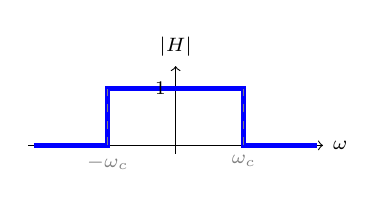
\begin{tikzpicture}[scale=0.72]
\draw[->] (-2.6,0) -- (2.6,0) node[right,font=\scriptsize] {$\omega$};
\draw[->] (0,-0.15) -- (0,1.4) node[above,font=\scriptsize] {$|H|$};
\draw[line width=1.8pt,blue] (-2.5,0) -- (-1.2,0) -- (-1.2,1) -- (1.2,1) -- (1.2,0) -- (2.5,0);
\draw[dashed,gray] (-1.2,0) node[below,font=\scriptsize] {$-\omega_c$} -- (-1.2,1);
\draw[dashed,gray] (1.2,0) node[below,font=\scriptsize] {$\omega_c$} -- (1.2,1);
\node[left,font=\scriptsize] at (0,1) {$1$};
\end{tikzpicture}
\end{center}
Passa frequências \textbf{abaixo} de $\omega_c$.

\column{0.48\textwidth}
\textbf{Passa-Altas (HP):}
\[
H_{HP}(\omega) = \begin{cases}
0, & |\omega| < \omega_c \\
1, & |\omega| \geq \omega_c
\end{cases}
\]
\vspace{-0.2cm}
\begin{center}
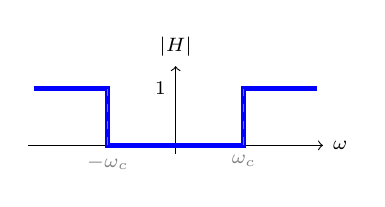
\begin{tikzpicture}[scale=0.72]
\draw[->] (-2.6,0) -- (2.6,0) node[right,font=\scriptsize] {$\omega$};
\draw[->] (0,-0.15) -- (0,1.4) node[above,font=\scriptsize] {$|H|$};
\draw[line width=1.8pt,blue] (-2.5,1) -- (-1.2,1) -- (-1.2,0) -- (1.2,0) -- (1.2,1) -- (2.5,1);
\draw[dashed,gray] (-1.2,0) node[below,font=\scriptsize] {$-\omega_c$} -- (-1.2,1);
\draw[dashed,gray] (1.2,0) node[below,font=\scriptsize] {$\omega_c$} -- (1.2,1);
\node[left,font=\scriptsize] at (0,1) {$1$};
\end{tikzpicture}
\end{center}
Passa frequências \textbf{acima} de $\omega_c$.
\end{columns}

\end{frame}

% ============================================

\begin{frame}{Tipos de Filtros Ideais: Passa-Faixas e Rejeita-Faixas}

\begin{columns}[T]
\column{0.48\textwidth}
\textbf{Passa-Faixas (BP):}
\[
H_{BP}(\omega) = \begin{cases}
1, & \omega_1 \!\leq\! |\omega| \!\leq\! \omega_2 \\
0, & \text{caso contrário}
\end{cases}
\]
\vspace{-0.2cm}
\begin{center}
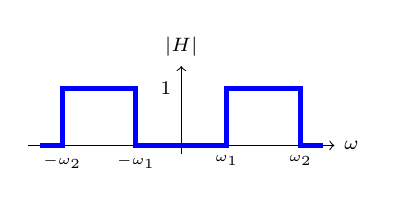
\begin{tikzpicture}[scale=0.72]
\draw[->] (-2.7,0) -- (2.7,0) node[right,font=\scriptsize] {$\omega$};
\draw[->] (0,-0.15) -- (0,1.4) node[above,font=\scriptsize] {$|H|$};
\draw[line width=1.8pt,blue]
  (-2.5,0) -- (-2.1,0) -- (-2.1,1) -- (-0.8,1) -- (-0.8,0)
  -- (0.8,0) -- (0.8,1) -- (2.1,1) -- (2.1,0) -- (2.5,0);
\node[below,font=\tiny] at (-2.1,0) {$-\omega_2$};
\node[below,font=\tiny] at (-0.8,0) {$-\omega_1$};
\node[below,font=\tiny] at (0.8,0) {$\omega_1$};
\node[below,font=\tiny] at (2.1,0) {$\omega_2$};
\node[left,font=\scriptsize] at (0,1) {$1$};
\end{tikzpicture}
\end{center}
Passa uma \textbf{faixa} entre $\omega_1$ e $\omega_2$.

\column{0.48\textwidth}
\textbf{Rejeita-Faixas (BS):}
\[
H_{BS}(\omega) = \begin{cases}
0, & \omega_1 \!<\! |\omega| \!<\! \omega_2 \\
1, & \text{caso contrário}
\end{cases}
\]
\vspace{-0.2cm}
\begin{center}
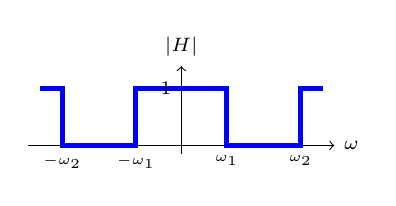
\begin{tikzpicture}[scale=0.72]
\draw[->] (-2.7,0) -- (2.7,0) node[right,font=\scriptsize] {$\omega$};
\draw[->] (0,-0.15) -- (0,1.4) node[above,font=\scriptsize] {$|H|$};
\draw[line width=1.8pt,blue]
  (-2.5,1) -- (-2.1,1) -- (-2.1,0) -- (-0.8,0) -- (-0.8,1)
  -- (0.8,1) -- (0.8,0) -- (2.1,0) -- (2.1,1) -- (2.5,1);
\node[below,font=\tiny] at (-2.1,0) {$-\omega_2$};
\node[below,font=\tiny] at (-0.8,0) {$-\omega_1$};
\node[below,font=\tiny] at (0.8,0) {$\omega_1$};
\node[below,font=\tiny] at (2.1,0) {$\omega_2$};
\node[left,font=\scriptsize] at (0,1) {$1$};
\end{tikzpicture}
\end{center}
\textbf{Bloqueia} uma faixa entre $\omega_1$ e $\omega_2$.
\end{columns}

\end{frame}

% ============================================

\begin{frame}{Características de Filtros Ideais}

\textbf{Propriedades dos filtros ideais:}

\begin{itemize}
\item \textbf{Banda passante:} $|H(\omega)| = 1$ (ganho unitário, sem atenuação)
\item \textbf{Banda de rejeição:} $|H(\omega)| = 0$ (atenuação infinita)
\item \textbf{Banda de transição:} Largura zero (mudança instantânea)
\item \textbf{Fase linear:} $\phi(\omega) = -\omega t_d$ na banda passante
\item \textbf{Seletividade perfeita:} Separa exatamente as frequências desejadas
\end{itemize}

\vspace{0.5cm}

\textbf{Aplicações teóricas:}
\begin{itemize}
\item Análise de sistemas de comunicação
\item Determinação de limites de desempenho
\item Referência para comparação com filtros reais
\end{itemize}

\vspace{0.3cm}

\textbf{Problema:} Filtros ideais são \textbf{fisicamente irrealizáveis}!

\end{frame}

% ============================================

\subsection{Problema da Causalidade}

\begin{frame}{Resposta ao Impulso do Filtro Passa-Baixas Ideal}

Já vimos que para $H_{LP}(\omega) = \rect(\omega/2\omega_c)$:

\[
h_{LP}(t) = \frac{\omega_c}{\pi} \sinc\left(\frac{\omega_c t}{\pi}\right) = \frac{\sin(\omega_c t)}{\pi t}
\]

\textbf{Análise da resposta:}

\begin{itemize}
\item Máximo em $t = 0$: $h_{LP}(0) = \omega_c/\pi$
\item Zeros em $t = \pm n\pi/\omega_c$ para $n = 1, 2, 3, ...$
\item \textbf{Existe para todo} $t \in (-\infty, \infty)$
\item Decai como $1/t$ (lentamente)
\end{itemize}

\vspace{0.3cm}

\textbf{Problema crítico:}

\[
h_{LP}(t) \neq 0 \quad \text{para} \quad t < 0
\]

O filtro responde \textbf{antes} do impulso ser aplicado!

\textbf{Conclusão:} Viola causalidade $\rightarrow$ fisicamente impossível.

\end{frame}

% ============================================

\begin{frame}{Critério de Paley-Wiener}

\textbf{Teorema (Paley-Wiener):}

Um filtro com função de transferência $H(\omega)$ é causalmente realizável se e somente se:

\[
\int_{-\infty}^{\infty} \frac{|\ln |H(\omega)||}{1 + \omega^2} d\omega < \infty
\]

\textbf{Consequências práticas:}

\begin{enumerate}
\item $|H(\omega)|$ não pode ser zero em nenhuma banda finita de frequências
\item A transição de banda passante para banda de rejeição deve ser gradual
\item $|H(\omega)|$ não pode cair a zero "rápido demais"
\end{enumerate}

\vspace{0.3cm}

\textbf{Para filtro ideal passa-baixas:}

$H(\omega) = 0$ para $|\omega| > \omega_c$ $\rightarrow$ $\ln|H(\omega)| = -\infty$

A integral diverge $\rightarrow$ \textbf{não satisfaz o critério} $\rightarrow$ não-causal.

\end{frame}

% ============================================

\begin{frame}{Aproximação de Filtros Ideais}

Como filtros ideais são irrealizáveis, usamos \textbf{aproximações causais}:

\textbf{Estratégias de aproximação:}

\begin{enumerate}
\item \textbf{Permitir banda de transição finita:}
   
   Mudança gradual entre passante e rejeição

\item \textbf{Permitir ondulação (ripple):}
   
   $|H(\omega)|$ não perfeitamente constante

\item \textbf{Atenuação finita na banda de rejeição:}
   
   $|H(\omega)| \neq 0$, mas muito pequeno

\item \textbf{Fase não perfeitamente linear:}
   
   Alguma distorção de fase aceitável
\end{enumerate}

\vspace{0.3cm}

\textbf{Compromissos inevitáveis:}

Não podemos ter simultaneamente: seletividade perfeita, causalidade, fase linear e complexidade finita.

\end{frame}

% ============================================

\subsection{Filtros Práticos}

\begin{frame}{Especificações de Filtros Práticos}

Um filtro prático passa-baixas é especificado por:

\begin{itemize}
\item \textbf{Banda passante:} $0 \leq \omega \leq \omega_p$
  \begin{itemize}
  \item Variação permitida: $1 - \delta_1 \leq |H(\omega)| \leq 1 + \delta_1$
  \item Ripple típico: $\delta_1 = 0.1$ (ondulação de 1 dB)
  \end{itemize}

\item \textbf{Banda de transição:} $\omega_p < \omega < \omega_s$
  \begin{itemize}
  \item Região onde $|H(\omega)|$ muda de passante para rejeição
  \item Quanto mais estreita, mais complexo o filtro
  \end{itemize}

\item \textbf{Banda de rejeição:} $\omega \geq \omega_s$
  \begin{itemize}
  \item Atenuação mínima: $|H(\omega)| \leq \delta_2$
  \item Atenuação típica: $\delta_2 = 0.01$ (40 dB)
  \end{itemize}
\end{itemize}

\vspace{0.3cm}

\textbf{Parâmetros de projeto:}
\begin{itemize}
\item Frequência de corte passante: $\omega_p$ ou $f_p$
\item Frequência de corte de rejeição: $\omega_s$ ou $f_s$
\item Ordem do filtro: $n$ (número de polos)
\end{itemize}

\end{frame}

% ============================================

\begin{frame}{Filtro de Butterworth}

O \textbf{filtro de Butterworth} maximiza a planura na banda passante.

\textbf{Função de transferência:}

\[
|H(\omega)|^2 = \frac{1}{1 + (\omega/\omega_c)^{2n}}
\]

onde $n$ é a ordem do filtro e $\omega_c$ é a frequência de corte de 3 dB.

\textbf{Propriedades:}

\begin{itemize}
\item Em $\omega = 0$: $|H(0)| = 1$ (ganho unitário em DC)
\item Em $\omega = \omega_c$: $|H(\omega_c)| = 1/\sqrt{2} \approx 0.707$ (-3 dB)
\item \textbf{Resposta maximally flat:} Primeiras $2n-1$ derivadas são zero em $\omega = 0$
\item Decaimento: $20n$ dB/década para $\omega \gg \omega_c$
\item Sem ondulação na banda passante ou de rejeição
\end{itemize}

\vspace{0.3cm}

\textbf{Características de fase:}
\begin{itemize}
\item Fase não-linear (especialmente próximo a $\omega_c$)
\item Distorção de fase presente
\end{itemize}

\end{frame}

% ============================================

\begin{frame}{Butterworth: Efeito da Ordem}

\[
|H(\omega)|^2 = \frac{1}{1 + (\omega/\omega_c)^{2n}}
\]

\textbf{Análise por ordem:}

\begin{itemize}
\item \textbf{$n = 1$:} Filtro RC simples, decaimento 20 dB/década
\item \textbf{$n = 2$:} Decaimento 40 dB/década, transição mais rápida
\item \textbf{$n \to \infty$:} Aproxima-se do filtro ideal (mas sempre causal)
\end{itemize}

\vspace{0.3cm}

\textbf{Relação ordem-transição:}

Para especificações dadas ($\omega_p$, $\omega_s$, $\delta_1$, $\delta_2$), a ordem necessária é:

\[
n \geq \frac{\log\left[\frac{(1/\delta_2)^2 - 1}{(1/\delta_1)^2 - 1}\right]}{2\log(\omega_s/\omega_p)}
\]

\vspace{0.3cm}

\textbf{Compromisso:} Maior ordem $\rightarrow$ melhor seletividade, mas maior complexidade e atraso.

\end{frame}

% ============================================

\begin{frame}{Filtro de Chebyshev Tipo I}

O \textbf{filtro de Chebyshev Tipo I} permite ondulação na banda passante para obter transição mais rápida.

\textbf{Função de transferência:}

\[
|H(\omega)|^2 = \frac{1}{1 + \epsilon^2 T_n^2(\omega/\omega_c)}
\]

onde:
\begin{itemize}
\item $T_n(x)$ é o polinômio de Chebyshev de ordem $n$
\item $\epsilon$ controla a ondulação na banda passante
\end{itemize}

\textbf{Propriedades:}

\begin{itemize}
\item \textbf{Ondulação equi-ripple} na banda passante: oscila entre 1 e $1/\sqrt{1+\epsilon^2}$
\item Banda de rejeição monótona (sem ondulação)
\item Decaimento mais rápido que Butterworth de mesma ordem
\item Para mesma seletividade, requer ordem menor que Butterworth
\end{itemize}

\textbf{Desvantagem:} Ondulação pode ser indesejável em algumas aplicações.

\end{frame}

% ============================================

\begin{frame}{Filtro de Chebyshev Tipo II (Inverso)}

O \textbf{filtro de Chebyshev Tipo II} permite ondulação na banda de rejeição.

\textbf{Características:}

\begin{itemize}
\item Banda passante monótona (sem ondulação)
\item Ondulação equi-ripple na banda de rejeição
\item Transição mais gradual que Tipo I
\item Zeros de transmissão na banda de rejeição
\end{itemize}

\vspace{0.5cm}

\textbf{Comparação dos tipos:}

\begin{center}
\small
\begin{tabular}{|l|c|c|}
\hline
\textbf{Característica} & \textbf{Tipo I} & \textbf{Tipo II} \\
\hline
Banda passante & Ondulação & Monótona \\
\hline
Banda de rejeição & Monótona & Ondulação \\
\hline
Transição & Mais rápida & Mais gradual \\
\hline
\end{tabular}
\end{center}

\end{frame}

% ============================================

\begin{frame}{Filtro de Bessel (Thomson)}

O \textbf{filtro de Bessel} maximiza a linearidade da fase.

\textbf{Objetivo:} Minimizar distorção de fase, ideal para pulsos.

\textbf{Propriedades:}

\begin{itemize}
\item \textbf{Fase aproximadamente linear} na banda passante
\item \textbf{Atraso de grupo aproximadamente constante:} $\tau_g(\omega) \approx \tau_0$
\item Resposta ao degrau com mínimo overshoot e ringing
\item Preserva melhor a forma de pulsos
\end{itemize}

\vspace{0.3cm}

\textbf{Desvantagem:}

\begin{itemize}
\item Seletividade pior que Butterworth ou Chebyshev
\item Para mesmas especificações, requer ordem maior
\item Banda de transição mais larga
\end{itemize}

\vspace{0.3cm}

\textbf{Aplicação ideal:} Transmissão de dados digitais onde preservar formato do pulso é crítico.

\end{frame}

% ============================================

\begin{frame}{Filtro Elíptico (Cauer)}

O \textbf{filtro elíptico} permite ondulação tanto na banda passante quanto na de rejeição.

\textbf{Características:}

\begin{itemize}
\item Ondulação equi-ripple em \textbf{ambas} as bandas
\item \textbf{Transição mais rápida} entre todas as aproximações
\item Para especificações dadas, requer a \textbf{menor ordem}
\item Zeros de transmissão na banda de rejeição e no eixo $j\omega$
\end{itemize}

\vspace{0.3cm}

\textbf{Função de transferência:}

\[
|H(\omega)|^2 = \frac{1}{1 + \epsilon^2 R_n^2(\omega/\omega_c)}
\]

onde $R_n$ é uma função racional (razão de polinômios).

\vspace{0.3cm}

\textbf{Aplicação:} Quando a ordem mínima é crítica (custo, consumo de energia).

\textbf{Desvantagem:} Fase muito não-linear, maior distorção de fase.

\end{frame}

% ============================================

\begin{frame}{Comparação Visual: Filtros Práticos de Ordem 4}

\begin{center}
\includegraphics[width=\figFull, height=0.72\textheight, keepaspectratio]{figures/cap3/filters_comparison}
\end{center}

\vspace{-0.3cm}
\begin{block}{Observação}
Butterworth: passante plana, sem ondulação. \quad Chebyshev: transição mais rápida. \quad Bessel: fase mais linear.
\end{block}

\end{frame}

% ============================================

\begin{frame}{Comparação de Aproximações de Filtros}

\textbf{Para mesma ordem $n$ e frequência de corte $\omega_c$:}

\begin{center}
\small
\begin{tabular}{|l|c|c|c|c|}
\hline
\textbf{Característica} & \textbf{Butter.} & \textbf{Cheby I} & \textbf{Bessel} & \textbf{Elíptico} \\
\hline
Planura passante & Boa & Ripple & Melhor & Ripple \\
\hline
Seletividade & Média & Boa & Fraca & Melhor \\
\hline
Fase linear & Média & Fraca & Melhor & Fraca \\
\hline
Ordem necessária & Média & Baixa & Alta & Mínima \\
\hline
Complexidade & Média & Média & Baixa & Alta \\
\hline
\end{tabular}
\end{center}

\vspace{0.5cm}

\textbf{Escolha do filtro depende da aplicação:}

\begin{itemize}
\item \textbf{Áudio:} Butterworth ou Bessel (fase linear)
\item \textbf{Comunicação digital:} Bessel (preserva pulsos)
\item \textbf{Separação espectral:} Chebyshev ou Elíptico (seletividade)
\item \textbf{Geral:} Butterworth (compromisso balanceado)
\end{itemize}

\end{frame}

% ============================================

\subsection{Relação Ordem-Desempenho}

\begin{frame}{Determinação da Ordem do Filtro}

\textbf{Problema:} Dadas especificações, determinar a ordem mínima necessária.

\textbf{Para filtro Butterworth passa-baixas:}

Especificações:
\begin{itemize}
\item Passante: $|H(\omega)| \geq 1 - \delta_1$ para $\omega \leq \omega_p$
\item Rejeição: $|H(\omega)| \leq \delta_2$ para $\omega \geq \omega_s$
\end{itemize}

A ordem necessária é:

\[
n = \left\lceil \frac{\log\left[\frac{(1/\delta_2)^2 - 1}{(1/\delta_1)^2 - 1}\right]}{2\log(\omega_s/\omega_p)} \right\rceil
\]

onde $\lceil \cdot \rceil$ é a função teto (arredondamento para cima).

\vspace{0.3cm}

\textbf{Simplificação prática:} Para $\delta_1, \delta_2 \ll 1$:

\[
n \approx \frac{\log(1/\delta_2) - \log(1/\delta_1)}{2\log(\omega_s/\omega_p)}
\]

\end{frame}

% ============================================

\begin{frame}{Exemplo: Projeto de Filtro Butterworth}

\textbf{Especificações:}

\begin{itemize}
\item Frequência de passante: $f_p = 1$ kHz
\item Frequência de rejeição: $f_s = 3$ kHz
\item Ondulação na passante: máx 1 dB ($\delta_1 = 0.1$, i.e., $|H| \geq 0.891$)
\item Atenuação na rejeição: mín 30 dB ($\delta_2 = 0.0316$, i.e., $|H| \leq 0.0316$)
\end{itemize}

\textbf{Cálculo da ordem:}

\[
n = \left\lceil \frac{\log[(1/0.0316)^2 - 1] - \log[(1/0.891)^2 - 1]}{2\log(3000/1000)} \right\rceil
\]

\[
= \left\lceil \frac{\log(1001) - \log(0.259)}{2\log(3)} \right\rceil = \left\lceil \frac{3.00 - (-0.587)}{2 \times 0.477} \right\rceil
\]

\[
= \left\lceil \frac{3.587}{0.954} \right\rceil = \lceil 3.76 \rceil = 4
\]

\textbf{Resultado:} Necessário filtro Butterworth de ordem 4.

\end{frame}

% ============================================

\begin{frame}{Implementação de Filtros}

\textbf{Formas de implementação:}

\begin{enumerate}
\item \textbf{Filtros analógicos (tempo contínuo):}
   \begin{itemize}
   \item Resistores, capacitores, indutores, amplificadores operacionais
   \item Implementação direta da função de transferência $H(s)$
   \item Limitados por componentes físicos
   \end{itemize}

\item \textbf{Filtros digitais (tempo discreto):}
   \begin{itemize}
   \item Algoritmos implementados em DSP, FPGA, software
   \item Versão discreta após conversão A/D
   \item Maior flexibilidade, estabilidade, reprodutibilidade
   \end{itemize}
\end{enumerate}

\vspace{0.3cm}

\textbf{Estruturas de implementação:}

\begin{itemize}
\item Cascata (série de seções de 2ª ordem)
\item Paralela (soma de seções)
\item Ladder (escada), para filtros passivos
\end{itemize}

\end{frame}

% ============================================

\begin{frame}{Resumo da Seção 3.5}

\textbf{Filtros ideais:}

\begin{itemize}
\item Seletividade perfeita, mas fisicamente irrealizáveis
\item Violam causalidade (critério de Paley-Wiener)
\item Servem como referência teórica
\end{itemize}

\vspace{0.3cm}

\textbf{Filtros práticos (aproximações causais):}

\begin{itemize}
\item \textbf{Butterworth:} Resposta plana, compromisso geral
\item \textbf{Chebyshev:} Ripple para maior seletividade
\item \textbf{Bessel:} Fase linear, preserva pulsos
\item \textbf{Elíptico:} Ordem mínima, máxima seletividade
\end{itemize}

\vspace{0.3cm}

\textbf{Compromissos inevitáveis:}

Seletividade $\leftrightarrow$ Fase linear $\leftrightarrow$ Complexidade

\textbf{Projeto:} Escolher aproximação e ordem baseado em especificações e aplicação.

\end{frame}
